\section{\ExercisePrefixEmbeddedC Beschleunigungssensor \optional}

Auf der Platine des FM4 Mikrocontrollers ist ein Beschleunigungssensor eingebaut, den du verwenden kannst um die Orientierung des Entwicklungsboards auszulesen. In der Library des Templates wird dir die Schnittstelle \lstinline|acceleration_app.h| zur Verfügung gestellt mit der du den Beschleunigungssensor für eine eigene Applikation verwenden kannst. In dieser Aufgabe wirst du ein Programm schreiben, mit dem du den Beschleunigungssensor nutzen kannst um eine digitale Wasserwaage zu simulieren. 
\begin{figure}[!htb]
	\centering
	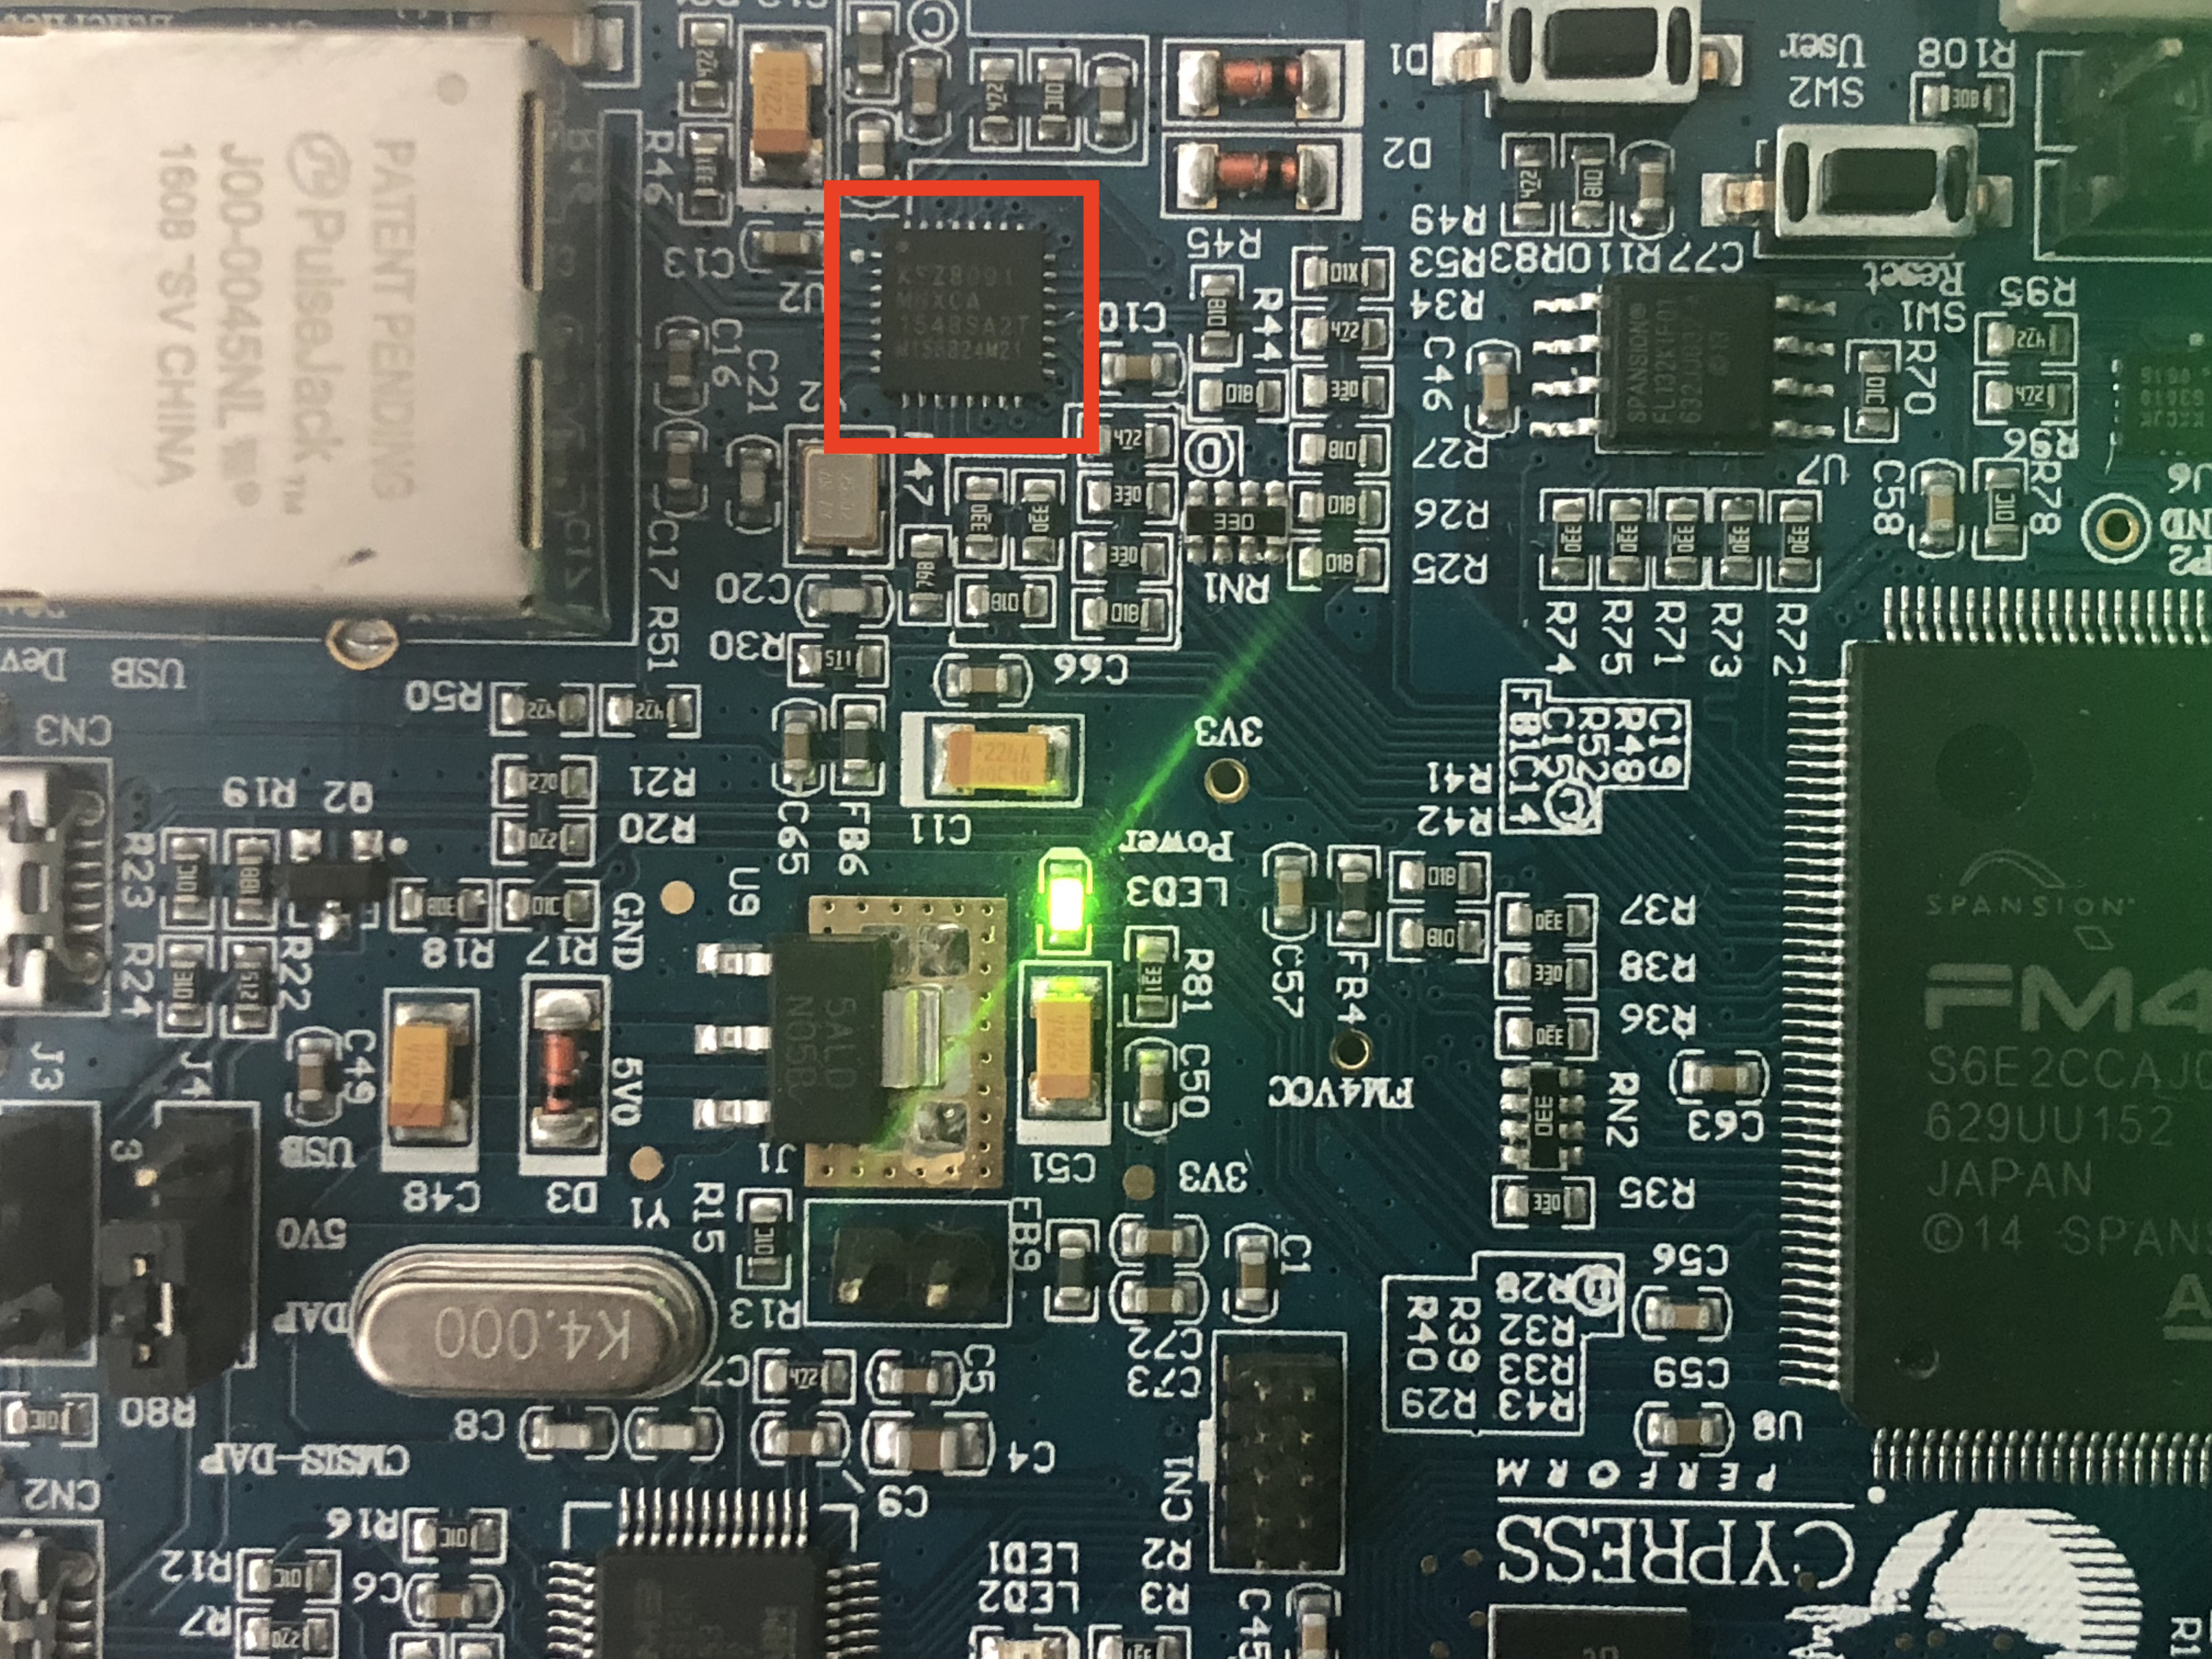
\includegraphics[width=0.4\textwidth]{./05_c/figures/kxcjk1013.jpg}
	\caption{Der Beschleunigungssensor des FM4-Boards}
	\label{fig:accelerometer}
\end{figure} 

In der Datei \lstinline|acceleration.c| findest du eine Vorlage für die Umsetzung einer Wasserwaage mithilfe des Beschleunigungssensors. In dieser fehlt noch die fertige Implementierung der Funktion \lstinline|cppp_rgbLEDAcceleration|. Bei der Initialisierung des Boards wird eine Interrupt-Routine gestartet, sobald neue Messdaten des Beschleunigungssensor des Chips vorliegen. Sofern die Routine ausgelöst wurde, wird \lstinline|cppp_accelerationDataAvailable| auf 1 gesetzt.  
In dem Array \lstinline|float cppp_orientationValues[3]| werden die aktuellen X-,Y- und Z-Achsen-Orientierungen des Boards in alphabetischer Reihenfolge gespeichert. 

\begin{enumerate}
	\item Gebe auf dem Display kontinuierlich die aktuelle Orientierung des Boards aus. Setze hierzu den Cursor per \lstinline|setCursor| an die Position \lstinline|(0,319)| und schreibe die Daten in diesem Format:
%	
	\cpppInputListing{05_c/listings/accelerometerLCDFormat.c}
%	
	\hints{
		\item Verwende zur Ausgabe von Variablen des Typs \lstinline|float| auf den Display die Funktion \lstinline|writeFloat(float value)|.
	}
%
	\item Nutze die Ergebnisse aus Teilaufgabe a) um ein Schema zu Erkennen, wann das Board sich nicht im Gleichgewicht befindet. Setze die RGB-LED auf Rot sofern sich das Board nicht im Gleichgewicht befindet und auf Grün sofern ja. Gebe ebenfalls eine Textausgabe gemäß dem Format oben auf dem Display aus, ob sich das Board im Gleichgewicht befindet. 
	\hints{
		\item Zum Ansteuern der RGB-LED kannst du in dieser Aufgabe als Vereinfachung die Library \lstinline|rgbled.h| verwenden. Hierzu muss zunächst die Funktion \lstinline|cppp_initLEDs| einmalig aufgerufen werden. Mit den Funktionen \lstinline|cppp_red/green/blueLEDOn/Off| kannst du die LEDs an oder ausschalten.
	}
\end{enumerate}

